\documentclass{standalone}

\usepackage{tikz}

\begin{document}

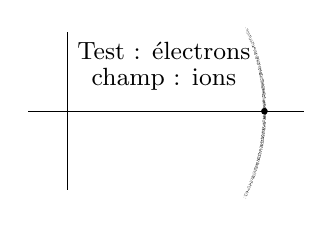
\begin{tikzpicture}

	\draw (0, -1) -- (0, 1) node[anchor = north west, align=left] {\small \shortstack{Test : électrons\\champ : ions}};
	
	\draw (-0.5, 0) -- (3, 0);
	
	\draw[ fill=black ] (2.5, 0) circle [ radius=0.035 ];
	
	\def\angle{25}
	\def\rayon{2.5}
	\def\width{0.02}
	\def\nangle{200}
	\pgfmathsetseed{\number\pdfrandomseed}
	\foreach \i in {-\nangle,...,\nangle} {
		\pgfmathsetmacro{\npoint}{5*rand*(exp(-1*\i/\nangle*\i/\nangle))}
		\pgfmathsetmacro{\npoint}{int(round(\npoint))}
    	\foreach \j in {0,..., \npoint} {
    		\pgfmathsetmacro{\effwidth}{rand*(\width)}%+0.75*\width*\i/\nangle)}
    		\pgfmathsetmacro{\effangle}{\i*\angle/\nangle+(rand-0.5)}
      		\fill[ black ] (\effangle:\rayon+\effwidth) circle [radius=0.0025];
    	}
    }
    

\end{tikzpicture}

\end{document}